
\section{Main-text material in full}\label{app:demoted}

This appendix keeps, verbatim, the tables, figures, and paragraphs of the
long-form manuscript that the main text summarizes.

\subsection{The two coupled choices in real data}
\begin{figure*}[t]
\centering
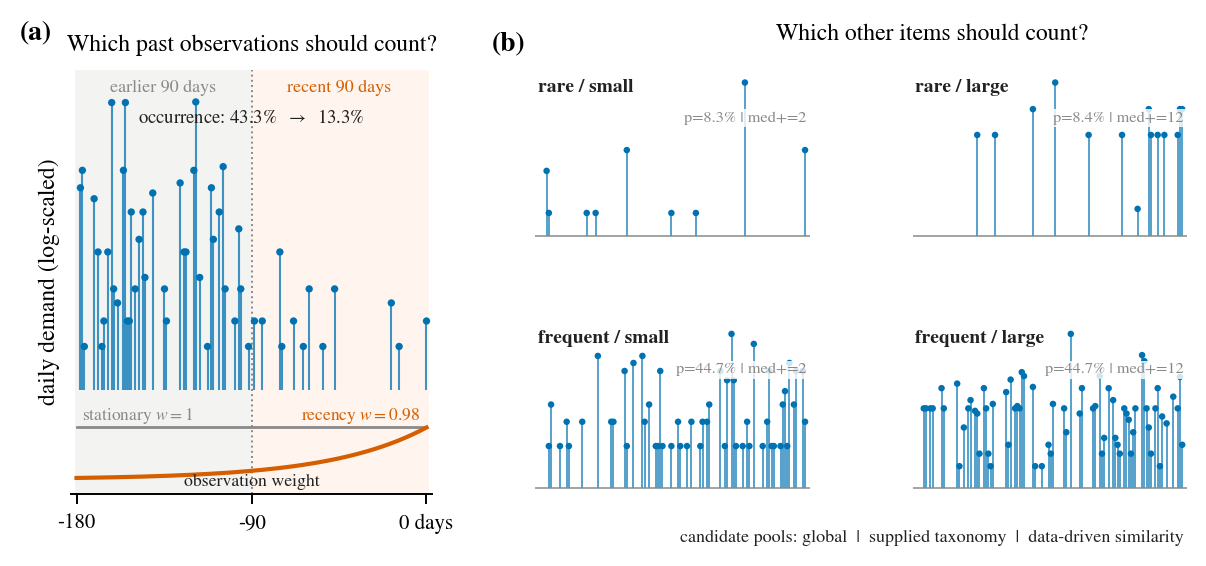
\includegraphics[width=0.98\textwidth]{fig01_problem.png}
\caption{The two coupled choices, in real intermittent demand.
\textbf{(a)} One item's daily history: occurrence falls from $43.3\%$ to
$13.3\%$ between the earlier and the recent ninety days, so a stationary
weighting ($w=1$) and a recency weighting ($w=0.98$) summarize the same
history differently---which past observations should count?
\textbf{(b)} Four items from the same panel, spanning rare and frequent
occurrence at small and large sizes: any pooled prior must decide which
of these heterogeneous neighbors an item should borrow strength
from---which other items should count? Candidate pools are a global
pool, a supplied taxonomy, and data-driven similarity.}
\label{fig:problem}
\end{figure*}

\subsection{Persistent prior leverage}

Fix an item and suppress its subscripts. Because
$n(w)=\sum_{t=1}^{T}w^{T-t}\le(1-w)^{-1}$ for $w<1$, the occurrence
credibility weight cannot converge to one.

\begin{proposition}[Forgetting keeps pooling relevant]
\label{prop:active}
For every horizon $T$,
$\lambda(w)\le\{1+(1-w)\phi\}^{-1}<1$ when $w<1$, whereas
$\lambda(1)\to1$ as $T\to\infty$. Hence the pooled occurrence prior
retains positive weight indefinitely under forgetting.
\end{proposition}

The statement is about leverage, not benefit: it does not guarantee
that a particular prior is a good shrinkage target. It says that the
choice of target can continue to affect forecasts even for old series.


\subsection{Resolution diagnostics recorded by the selector}
Fitting each candidate already produces everything the resolution
analysis of Section~\ref{sec:resolution} needs, so the selector records it
rather than recomputing it later. For every $(r,w)$ and every resulting
group $g$ we store, from the fitting head only, the median occurrence and
positive-size credibility weights $\lambda_i^{(o)}$ and $\lambda_i^{(+)}$,
the share of items with $\lambda_i^{(+)}<0.1$, the group sizes $m_g$, and
the resolution statistic
\[
\hat z_g=\frac{S_g^2-\bar s_g}{\sqrt{2/(m_g-1)}\,S_g^2},
\]
whose nonpositive values coincide with the collapse event
$\hat\tau_g^2=0$ of Proposition~\ref{prop:twosided}. These quantities cost
nothing beyond the fit that produced them, they are computed before any
external observation is seen, and they answer a question the validation
score cannot: not which candidate scores best on the tail, but whether the
discounted data contain enough information to estimate the candidate's
group structure at all. Section~\ref{sec:main-results} uses them to
separate the two. The full selection surface and the accompanying
diagnostics are released with every run
(\texttt{remix\_selection\_diagnostics.csv}).


\subsection{Pooling candidates and computational profile}
Let $\mathcal R$ contain three ways to construct $g(\cdot)$ from the
fitting data. Table~\ref{tab:pool-candidates} orders them from coarse to
fine: one prior for the panel, one prior per fixed demand-pattern class,
and one prior per learned component. The ladder is deliberate. The
question this paper asks is not which rung is best in general---that
depends on the panel---but whether the discounted data support moving up
it at all. Section~\ref{sec:resolution} gives the condition under which
they do, and Section~\ref{sec:main-results} reports what happens when they
do not.

\begin{table}[t]
\centering
\caption{Pooling candidates used by \EBB{}, ordered coarse to fine.
Every data-dependent label is computed from the selector's fitting head,
never its validation tail.}
\label{tab:pool-candidates}
\small
\setlength{\tabcolsep}{3.5pt}
\begin{tabular}{lp{0.70\linewidth}}
\toprule
Candidate & Shared-prior groups\\
\midrule
Global & All items share one prior.\\
Taxonomy & Four ADI/CV$^2$ demand-pattern classes (smooth, intermittent,
erratic, lumpy) using the classical thresholds $1.32$ and $0.49$
\citep{syntetos2005categorization}.\\
Learned & Hard assignments from a mixture of occurrence--size prior
components; $K\in\{1,\ldots,6\}$ is selected by BIC.\\
\bottomrule
\end{tabular}
\end{table}

For the learned candidate, component $k$ carries
$\eta_k=(\alpha_k,\beta_k,\mu_{0,k},\tau_k^2,\sigma_k^2)$. Its item
marginal is the product of Beta--Binomial occurrence evidence and Normal
random-effects size evidence. EM has an analytic responsibility update;
its M-step maximizes responsibility-weighted EB objectives. A
deterministic quantile initialization makes repeated fits seed-free.
Mixture labels are built once from the fitting head and shared across the
discount grid, with $K\in\{1,\dots,6\}$ selected by BIC at that fit.
Re-learning the partition separately at every discount is a natural
variant---changing $w$ changes both the item evidence and the components
it can support---but we do not evaluate it here. The
selected responsibilities are converted to hard labels so all three
candidates share the same downstream forecaster.



Two properties of this cost profile matter for the comparisons that
follow. First, the whole pipeline is CPU-only and closed form apart from
the mixture search: fitting and predicting a panel costs on the order of
milliseconds per series, so the full 24-candidate joint selection
completes in minutes on a laptop-class machine and no GPU, tuning budget,
or convergence diagnostic is required. Second, estimation is exact rather
than approximate at every stage, so repeated end-to-end runs are
bit-identical in the released test suite. Neither property is an accuracy
claim; both are the terms on which the accuracy results in
Section~\ref{sec:experiments} should be read, since several of the
strongest comparators there cost two to three orders of magnitude more per
series and none is reproducible to the bit. Measured wall-clock figures
for every method are in Appendix~\ref{app:implementation}.

\subsection{Fixed-origin results in full}
\label{sec:main-results}
% =========================================================================

\begin{table*}[t]
\centering
\caption{\textbf{Probabilistic forecasting is the primary comparison.}
Scaled pinball loss (SPL; lower is better) is reported as the mean over
$q\in\{0.1,0.25,0.5,0.75,0.9\}$ and at q90. Bold and underline mark the
best and second-best non-degenerate methods. M5 reports seed 42 for direct
comparability; three-seed robustness is summarized in the text. \EBB{}
uses its raw predictive law, with no post-hoc calibration. TweedieGP is the
official implementation of Damato et al.\ at its released defaults on
all five panels; Appendix~\ref{app:efficiency} reports measured cost.
The all-zero row is a metric diagnostic and
is excluded from ranking.}
\label{tab:prob}
\small
\setlength{\tabcolsep}{3.2pt}
\begin{tabular}{lcc@{\hspace{9pt}}cc@{\hspace{9pt}}cc@{\hspace{9pt}}cc@{\hspace{9pt}}cc}
\toprule
 & \multicolumn{2}{c}{Online Retail} & \multicolumn{2}{c}{M5} & \multicolumn{2}{c}{Auto} & \multicolumn{2}{c}{Carparts} & \multicolumn{2}{c}{RAF}\\
\cmidrule(lr){2-3}\cmidrule(lr){4-5}\cmidrule(lr){6-7}\cmidrule(lr){8-9}\cmidrule(lr){10-11}
Model & Mean & q90 & Mean & q90 & Mean & q90 & Mean & q90 & Mean & q90\\
\midrule
AutoARIMA & 1.0069 & 1.6297 & 1.7919 & 2.4148 & 0.3189 & 0.2659 & 0.4084 & 0.4897 & 0.4020 & 0.5910\\
AutoTheta & 1.0055 & 1.6056 & 1.7954 & 2.3123 & 0.3403 & 0.2760 & 0.3925 & \secondbest{0.4697} & 0.4104 & 0.5956\\
CP-Croston & 1.5502 & 2.7686 & 1.6902 & \best{2.1551} & 0.3260 & 0.3105 & 0.4012 & 0.5433 & 0.3322 & 0.4927\\
CP-SBA & 1.5492 & 2.8601 & 1.6939 & 2.1736 & 0.3256 & 0.3153 & 0.3982 & 0.5418 & 0.3290 & 0.4920\\
CP-TSB & 1.1744 & 2.6746 & 1.8794 & 2.3148 & 0.3459 & 0.3150 & 0.3783 & 0.4842 & 0.3814 & 0.4986\\
CP-ADIDA & 1.1239 & 2.5409 & 1.7150 & 2.1949 & 0.3275 & 0.3082 & 0.3571 & 0.4982 & 0.3097 & 0.4905\\
CP-IMAPA & 1.1280 & 2.5506 & 1.7190 & 2.1904 & 0.3279 & 0.3084 & 0.3561 & 0.4908 & 0.3116 & 0.4907\\
Tweedie-GLM & 1.1477 & 1.7458 & 4.0693 & 5.2620 & 0.3221 & 0.2783 & 0.4776 & 0.6897 & 0.3121 & 0.5312\\
iETS & 0.9846 & 1.7544 & 2.0282 & 2.9772 & 0.3448 & 0.3252 & 0.4561 & 0.5646 & 0.3494 & \secondbest{0.4900}\\
TweedieGP & \best{0.8845} & \best{1.5218} & \best{1.6228} & \secondbest{2.1723} & \secondbest{0.2985} & \best{0.2598} & \best{0.3214} & \best{0.4600} & \secondbest{0.2763} & 0.5219\\
\midrule
Zero (diagnostic) & 0.9161 & 1.6490 & 1.9590 & 3.5262 & 0.5612 & 1.0102 & 0.3736 & 0.6725 & 0.2669 & 0.4805\\
\midrule
\EBB{} (ours) & \secondbest{0.8849} & \secondbest{1.5268} & \secondbest{1.6707} & 2.4758 & \best{0.2937} & \secondbest{0.2599} & \secondbest{0.3229} & 0.4817 & \best{0.2680} & \best{0.4856}\\
\bottomrule
\end{tabular}
\end{table*}

Table~\ref{tab:prob} sets the empirical position, and it is a narrow one.
\EBB{} attains the lowest mean SPL on Auto and RAF, by $1.6\%$ and
$3.0\%$ over the official TweedieGP implementation, both significant
(Table~\ref{tab:spl-significance}); TweedieGP attains it on Online Retail,
Carparts, and M5, by $0.05\%$, $0.5\%$, and $2.9\%$, of which only the M5
margin is significant. Against every other comparator \EBB{} is best on
all five panels, by $10.1\%$ over iETS on Online Retail and $1.2\%$ over
CP-Croston on M5. Across three independent
5{,}000-series M5 samples the selected configuration is identical---%
$(\text{mixture},\,w{=}0.95,\,K{=}6)$---and \EBB{} has mean SPL
$1.7501\pm0.084$ against $1.7547\pm0.065$ for CP-Croston, its closest
comparator: ahead on two samples, behind by $1.0\%$ on the third, and
ahead on average by $0.3\%$, well within one standard deviation. We report
the spread rather than an aggregate win because it is the quantity
Section~\ref{sec:leverage} explains. The explanation is not that these
panels leave no room for a hierarchical construction to work; on three of
them the credibility weights say otherwise. It is that the room which
exists is not converted by a learned partition, which is why the
achievable margin is set by the shared predictive law rather than by the
pooling structure.

The degenerate row exposes what the central quantiles cannot see. On RAF,
the all-zero forecast is marginally better through q90 because the true
quantiles of most series are zero. At $q\in\{0.95,0.975,0.99\}$ it falls
behind every intensity-bearing method, and intensity-bearing models become
distinguishable from one another (Appendix~\ref{app:fartail}). TweedieGP
is strongest throughout the Carparts far tail and remains competitive on
RAF. The probabilistic claim is therefore not that one distribution wins
every quantile, but that \EBB{} is the most consistent aggregate
performer across panels and remains informative in the region where a zero
forecast ceases to be useful.

Point forecasts tell a deliberately weaker story. \EBB{} is best on six
of ten MAE/RMSSE cells and top two on seven, but the zero forecast has the
lowest MAE on three panels and classical methods lead several remaining
cells. We report the complete point table and horizon decomposition in
Appendix~\ref{app:point}: they establish competitiveness and rule out a
long-horizon averaging artifact, but do not support uniform point-forecast
superiority.

% =========================================================================


\subsection{Walk-forward results in full}
\label{sec:walkforward}
% =========================================================================

\begin{table*}[t]
\centering
\caption{\textbf{Strict probabilistic walk-forward evaluation on all five
panels.} Online Retail and M5 use seven-day blocks; Auto, Carparts, and
RAF use monthly blocks. Mean and q90 are scaled pinball losses; all five
quantiles, coverage, and interval width are reported in
Appendix~\ref{app:walkforward}. Classical wrappers and ACI refit each
block. AutoARIMA, AutoTheta, iETS, and TweedieGP refit every four blocks
on Online Retail and every block on the monthly panels; on M5 these four
were not run under this protocol on cost grounds (dashes). \EBB{} updates
sufficient statistics each block; ACI-\EBB{} applies the ACI-ADIDA
calibration layer to \EBB{}'s predictive quantiles, and \EBB{} (rule)
applies it only where the validation-tail rule selects it, so it equals
one of the two rows above it on each panel and is not ranked. Bold and underline
rank non-degenerate methods by SPL; on RAF the all-zero forecast is
marginally lower than every method through q90. On M5, the longest daily
panel, the adaptive conformal layer decides the ranking: ACI-\EBB{} leads,
ACI-ADIDA is second, and uncalibrated \EBB{} is third.}
\label{tab:wfprob}
\footnotesize
\setlength{\tabcolsep}{3.0pt}
\begin{tabular}{lrrrrrrrrrr}
\toprule
 & \multicolumn{2}{c}{Online Retail} & \multicolumn{2}{c}{Carparts} & \multicolumn{2}{c}{Auto} & \multicolumn{2}{c}{RAF} & \multicolumn{2}{c}{M5}\\
\cmidrule(lr){2-3}\cmidrule(lr){4-5}\cmidrule(lr){6-7}\cmidrule(lr){8-9}\cmidrule(lr){10-11}
Model & Mean & q90 & Mean & q90 & Mean & q90 & Mean & q90 & Mean & q90\\
\midrule
AutoARIMA & 1.0627 & 1.5225 & 0.4195 & 0.4839 & 0.3139 & 0.2632 & 0.4083 & 0.5920 & --- & ---\\
AutoTheta & 1.0586 & 1.4835 & 0.4056 & 0.4743 & 0.3224 & 0.2619 & 0.4308 & 0.6233 & --- & ---\\
iETS & 1.1092 & 1.9404 & 0.4362 & 0.5154 & 0.3286 & 0.3009 & 0.3537 & 0.4902 & --- & ---\\
CP-TSB & 1.3733 & 2.8422 & 0.3836 & 0.4758 & 0.3297 & 0.3009 & 0.3842 & 0.4941 & 1.6616 & 2.0422\\
CP-ADIDA & 1.1576 & 2.5143 & 0.3509 & 0.4880 & 0.3175 & 0.2949 & 0.3095 & \secondbest{0.4894} & 1.5537 & 1.9629\\
CP-IMAPA & 1.1773 & 2.5224 & 0.3492 & 0.4789 & 0.3176 & 0.2948 & 0.3127 & 0.4903 & 1.5457 & 1.9490\\
ACI-ADIDA & 0.9108 & 1.6681 & 0.3417 & 0.4767 & 0.3147 & 0.2900 & 0.3085 & 0.5598 & \secondbest{1.4192} & \secondbest{1.8064}\\
TweedieGP & \best{0.8526} & \best{1.3791} & \best{0.3121} & \best{0.4326} & 0.2924 & \best{0.2539} & 0.2801 & 0.5261 & --- & ---\\
Zero (diagnostic) & 0.9161 & 1.6490 & 0.3736 & 0.6725 & 0.5612 & 1.0102 & 0.2669 & 0.4805 & 1.9590 & 3.5262\\
\midrule
\EBB{} & \secondbest{0.8540} & \secondbest{1.4002} & 0.3145 & 0.4578 & \secondbest{0.2910} & 0.2563 & \best{0.2681} & \best{0.4864} & 1.4851 & 1.8797\\
ACI-\EBB{} & 0.9082 & 1.5623 & \secondbest{0.3128} & \secondbest{0.4521} & \best{0.2901} & \secondbest{0.2560} & \secondbest{0.2743} & 0.5175 & \best{1.3785} & \best{1.6438}\\
\EBB{} (rule) & 0.8540 & 1.4002 & 0.3145 & 0.4578 & 0.2901 & 0.2560 & 0.2681 & 0.4864 & 1.3785 & 1.6438\\
\bottomrule
\end{tabular}
\end{table*}

Table~\ref{tab:wfprob} is the deployment-facing test, and it reproduces
the fixed-origin picture for the uncalibrated methods. \EBB{} leads on
Auto and RAF, by $0.5\%$ and $4.3\%$ over TweedieGP; TweedieGP leads on
Online Retail and Carparts by $0.2\%$ and $0.8\%$. Per-series paired tests
(Table~\ref{tab:wf-significance}) cannot separate the two on Online
Retail, Carparts, or Auto, and favor \EBB{} on RAF. Over adaptive
conformal inference on ADIDA, \EBB{} gains $6.2\%$ on Online Retail and
$8.0\%$ on Carparts, beats every static conformal wrapper on all five
panels, and loses M5 by $4.4\%$.

The M5 loss is a calibration effect, and the same layer is available to
\EBB{}. ACI-\EBB{} reads \EBB{}'s predictive quantile at the adaptive
level instead of the nominal one. On M5 it lowers mean SPL from $1.4851$
to $1.3785$, $2.9\%$ below ACI-ADIDA and significant; it also leads Auto
($0.2901$) and brings Carparts to within $0.2\%$ of TweedieGP. On Online
Retail and RAF the same layer hurts, by $6.3\%$ and $2.3\%$, because the
per-series coverage signal is too noisy on those panels to improve an
already calibrated forecaster. Whether to apply it is therefore a
selection problem, and the initialization window already answers it: on
the same 80/20 chronological split used to select the discount, \EBB{} is
walked forward over the validation tail with and without the layer, and
the layer is applied iff its tail pinball is lower
(Appendix~\ref{tab:aci-rule}). The rule applies the layer on M5 and Auto
and withholds it elsewhere, matching the ex-post better variant on
4 of five panels (Carparts is the exception, where the two
are within $0.5\%$ and statistically undecided), and the tail gains it
sees track the external ones ($+7.8\%$ versus $+7.2\%$ on M5, $-7.9\%$
versus $-6.3\%$ on Online Retail). The resulting row, \EBB{} (rule), is
within 0.8\% ({Carparts}) of the best competing method on every
panel under walk-forward updating. Two further facts survive the mixed
result: under equal calibration \EBB{} beats the ADIDA base on all five
panels (undecided only on Online Retail), and the adaptive layer's benefit
is a property of the panel, not of the forecaster it wraps.

Table~\ref{tab:regret} and Figure~\ref{fig:frontier} summarize both
protocols by the largest shortfall to the per-panel best. Against
competing methods, \EBB{} and TweedieGP are the only ones within five
percent everywhere (\EBB{} at most $3.0\%$ at fixed origin and $4.6\%$
under walk-forward updating; TweedieGP $3.1\%$ and $4.5\%$), and every
other method is at least $15\%$ behind on some panel. Counting our own
wrapper as a competitor, uncalibrated \EBB{} trails ACI-\EBB{} by $7.7\%$
on M5, and \EBB{} (rule) closes that to 0.8\%. The two leaders differ in cost. TweedieGP refits per-series
variational GPs at every update, so its walk-forward runs took between
$36$ minutes (Auto) and $2.4$ hours (RAF) with twelve workers and project
to about $51$ hours on M5 at the Online Retail cadence; \EBB{} updates
sufficient statistics in closed form and completes each of the five
walk-forward runs in under $40$ seconds on one core, and ACI-\EBB{} adds
a few seconds (Table~\ref{tab:wfcost}).

\begin{table}[t]
\centering
\caption{\textbf{Largest shortfall to the per-panel best.} For each
method, the maximum over panels of its mean-SPL regret to the best
non-degenerate method on that panel (percent; the panel attaining it in
parentheses; Carp.\ is Carparts), and the number of panels on which the method is within
$5\%$ of the best. A superscript gives the number of panels evaluated
when fewer than five. ACI-\EBB{} and the rule row exist only under walk-forward updating; the
rule row is excluded from the per-panel best.
Per-panel regrets are in Table~\ref{tab:regret-full}.}
\label{tab:regret}
\footnotesize
\setlength{\tabcolsep}{2.6pt}
\begin{tabular}{lcccc}
\toprule
 & \multicolumn{2}{c}{Fixed origin} & \multicolumn{2}{c}{Walk-forward}\\
\cmidrule(lr){2-3}\cmidrule(lr){4-5}
Method & Max (panel) & $\le5\%$ & Max (panel) & $\le5\%$\\
\midrule
AutoARIMA & 50.0 (RAF) & 0/5 & 52.3 (RAF)$^{4}$ & 0/4\\
AutoTheta & 53.1 (RAF) & 0/5 & 60.7 (RAF)$^{4}$ & 0/4\\
Tweedie-GLM & 150.8 (M5) & 0/5 & --- & ---\\
iETS & 41.9 (Carp.) & 0/5 & 39.8 (Carp.)$^{4}$ & 0/4\\
CP-Croston & 75.3 (OR) & 1/5 & 60.9 (OR) & 0/5\\
CP-SBA & 75.1 (OR) & 1/5 & 61.5 (OR) & 0/5\\
CP-TSB & 42.3 (RAF) & 0/5 & 61.1 (OR) & 0/5\\
CP-ADIDA & 27.1 (OR) & 0/5 & 35.8 (OR) & 0/5\\
CP-IMAPA & 27.5 (OR) & 0/5 & 38.1 (OR) & 0/5\\
ACI-ADIDA & --- & --- & 15.1 (RAF) & 1/5\\
TweedieGP & 3.1 (RAF) & 5/5 & 4.5 (RAF)$^{4}$ & 4/4\\
\midrule
\EBB{} & 3.0 (M5) & 5/5 & 7.7 (M5) & 4/5\\
ACI-\EBB{} & --- & --- & 6.5 (OR) & 4/5\\
\EBB{} (rule) & --- & --- & 0.8 (Carp.) & 5/5\\
\bottomrule
\end{tabular}
\end{table}

\begin{figure*}[t]
\centering
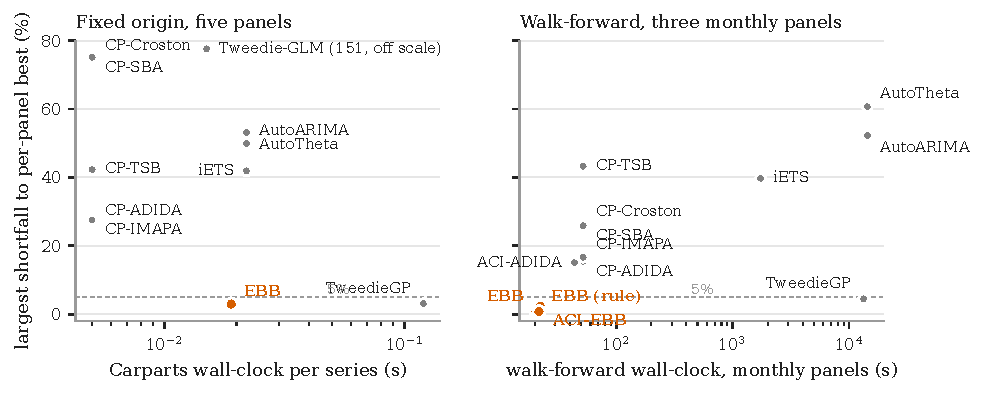
\includegraphics[width=0.96\textwidth]{figs/fig12_frontier.pdf}
\caption{\textbf{Largest shortfall against cost.} Each point is one
method; $y$ is its largest mean-SPL shortfall to the per-panel best
(Table~\ref{tab:regret}), $x$ is measured wall-clock on a log scale.
Left: fixed origin over five panels against Carparts cost per series
(Table~\ref{tab:efficiency}). Right: walk-forward over the three monthly
panels, on which every method has a measured wall-clock, against the total
walk-forward wall-clock on those panels (Table~\ref{tab:wfcost}; TweedieGP
uses twelve workers, every other method one process). The dashed line
marks $5\%$.}
\label{fig:frontier-full}
\end{figure*}



The configuration is selected once at the origin and then updated online;
repeated online re-selection is outside the present experiment.

% =========================================================================


\subsection{Controlled test of the resolution mechanism}

\label{sec:synthetic}
% =========================================================================

Real data never reveal the true pooling partition, so on their own they
cannot distinguish a partition that is not worth having from one we failed
to find. Both appear as a small number. We therefore construct panels
where the partition is correct by definition, and use them as a reference
against which the learned partitions of Section~\ref{sec:leverage} are
measured: what a good partition is worth at a given level of credibility
leverage, rather than what our estimator obtains there.

We simulate from the hierarchical hurdle model of \eqref{eq:model} with
group centers arranged symmetrically around a fixed grand mean, so that
increasing separation does not change the panel scale. Each cell compares
a single pool against the known true partition under the same predictive
representation, with nine paired replicates, and sweeps the two quantities
that Section~\ref{sec:resolution} identifies as controlling credibility:
the discount $w$ and the series length $T$. The resulting grid spans the
leverage range the real panels occupy, from the near-fully-shrunk regime
of Carparts to the item-dominated regime of Auto and RAF.

\begin{table*}[t]
\centering
\caption{Advantage of the \emph{true} partition over a single pool on
simulated panels (mean percentage improvement over nine paired replicates;
standard error in parentheses). Positive favors the partition. $T$ is
series length.}
\label{tab:sanity}
\small
\setlength{\tabcolsep}{3.5pt}
\begin{tabular}{llrrrr}
\toprule
$T$ & $w$ & NLL & log-size MSE & pinball & MAE\\
\midrule
$30$ & $0.90$ & $2.40\;(0.18)$ & $17.15\;(2.39)$ & $2.25\;(0.61)$ & $-1.72\;(0.73)$\\
$30$ & $0.95$ & $1.12\;(0.39)$ & $9.00\;(2.45)$ & $-0.44\;(0.58)$ & $-0.17\;(0.51)$\\
$30$ & $1.00$ & $1.02\;(0.08)$ & $8.37\;(1.53)$ & $-0.69\;(0.32)$ & $-1.95\;(0.59)$\\
$120$ & $0.90$ & $1.65\;(0.22)$ & $18.36\;(1.56)$ & $1.57\;(0.64)$ & $-3.34\;(1.37)$\\
$120$ & $0.95$ & $0.96\;(0.11)$ & $3.65\;(0.77)$ & $0.23\;(0.28)$ & $-1.32\;(0.73)$\\
$120$ & $1.00$ & $0.23\;(0.04)$ & $1.13\;(0.31)$ & $-0.32\;(0.13)$ & $-0.80\;(0.11)$\\
\bottomrule
\end{tabular}
\end{table*}

Table~\ref{tab:sanity} gives the result. The true partition improves NLL
and log-size MSE in every cell, and pinball loss whenever forgetting is
strong; in a separate length sweep its pinball advantage decays from
$1.53\%$ at $T=12$ to $0.01\%$ at $T=400$. Both patterns follow the
credibility mechanism directly. Discounting or short histories reduce an
item's own weight $\lambda^{(+)}_i$ and open room for a prior to act;
long undiscounted histories drive $\lambda^{(+)}_i\to1$ and make every
partition irrelevant. Stronger forgetting simultaneously makes group
variance components harder to estimate, as
Proposition~\ref{prop:twosided} predicts, which is why the gains in the
$w=0.90$ rows are bought against a noisier $\hat\tau_g^2$ and do not
continue to grow without limit. Extending the grid with a separation axis
(Appendix~\ref{app:simulation-details}; group centers $0$ to $3$
log-units apart) shows that the return is governed by the forgetting
regime as much as by leverage: with no separation in either block the return is within noise of
zero; with $w=0.90$ a true partition earns $1$--$2.7\%$ from separation
$0.5$ upward, with $w=0.95$ it exceeds $1\%$ only at separation $0.5$
with long histories ($\lambda^{(+)}\approx0.4$), and with $w=1$ it never
does. The learned mixture, run on the same simulated panels, is negative
at every moderate separation, and the two remedies already in the code
base---label sample-splitting and credibility shrinkage of the group
variance---do not recover the loss (grid means $-0.58\%$, $-0.79\%$, $-0.66\%$, and $-0.56\%$ combined).

MAE moves the other way in all six cells. A known-correct partition, on
data generated from the model it describes, is reported as harmful by the
metric most commonly used in this literature. We take this as the cleanest
available statement of why Section~\ref{sec:main-results} treats
absolute-error criteria as diagnostics rather than as the headline.

\paragraph{What these panels are for.}
Plotted against median $\lambda^{(+)}$, the cells of
Table~\ref{tab:sanity} and the length sweep trace the grey curves of
Figure~\ref{fig:refinement-leverage}: the return to \emph{correct}
structure as a function of leverage. Because the partition is supplied
rather than estimated, that return is an upper envelope---no procedure
that must also learn the grouping can exceed it, and any procedure that
falls below it is losing something to estimation rather than to a lack of
structure. This is the comparison Section~\ref{sec:leverage} draws, and it
is the reason the controlled study is necessary rather than decorative:
the real panels supply the leverage coordinates, and only a known-partition
experiment can supply the ordinate they should be judged against.

Two boundaries apply. The experiment isolates the value of correct
structure and says nothing about whether the mixture recovers it---indeed
Section~\ref{sec:leverage} shows it does not, and the gap between the two
is precisely what the comparison measures. And it simulates from the model
that \EBB{} fits, so the mechanism is tested under correct specification
only; a misspecified size law would shift the envelope, though it is hard
to see how it would raise it. Full diagnostics, including the growth of
$\mathrm{RMSE}(\hat\tau_g^2)$ as $w$ falls, are in
Appendix~\ref{app:simulation-details}.

% =========================================================================


\subsection{Leverage, selection, and ablation}
\label{sec:leverage}
% =========================================================================

The results so far are consistent and small. This section asks whether
their size is a property of the data or of our estimator, and shows that
the two can be told apart with quantities the selector already computes on
the fitting head (Section~\ref{sec:select}).

\paragraph{What gets selected, and how weakly.}
All five panels select $w<1$: Carparts $0.90$, Online Retail and M5
$0.95$, Auto $0.99$, and RAF $0.997$. Across three independent
5{,}000-series M5 samples the selected configuration is identical in
structure, discount, and mixture order---$(\text{mixture},\,w{=}0.95,\,
K{=}6)$ in every case.

The pooling axis behaves differently, and the honest summary is that it
barely resolves. On three panels the spread between the best and worst
pooling structure at the selected discount is under a tenth of a percent
of validation SPL: $0.05\%$ on Online Retail, $0.08\%$ on Carparts,
$0.02\%$ on RAF. Only two panels separate at all---M5, where the learned
mixture beats the global pool by $0.58\%$, and Auto, where the global pool
beats every refinement by $0.31\%$. Announcing a winner on the other three
would report selector noise. What the selector reliably does is choose a
discount and avoid poor structural corners; it does not discover demand
taxonomies, and we do not claim it does.

\begin{table*}[t]
\centering
\caption{\textbf{Credibility leverage under a single pool.} Median
credibility weight per panel at no forgetting and at the selected
discount, for both blocks of the hurdle model:
$\lambda^{(o)}_i=n_i/(n_i+\phi_g)$ for occurrence and
$\lambda^{(+)}_i=n_i^{+}/(n_i^{+}+\kappa_g)$ for positive size, the
latter being the quantity bounded by Proposition~\ref{prop:twosided}.
A weight near one means the item's own history dominates its posterior,
bounding how far any shared prior can move it. ``$<0.1$'' is the share of
items whose size-block weight falls below $0.1$. The final column is the
external MAE change of a separately selected learned partition relative to
the single pool; negative favors the single pool.}
\label{tab:leverage}
\small
\setlength{\tabcolsep}{3.0pt}
\begin{tabular}{lccccccc}
\toprule
 & & \multicolumn{3}{c}{$\lambda^{(+)}$ (size)} & \multicolumn{2}{c}{$\lambda^{(o)}$ (occ.)} & learned\\
\cmidrule(lr){3-5}\cmidrule(lr){6-7}
Panel & $w^{*}$ & $w{=}1$ & $w^{*}$ & $<0.1$ & $w{=}1$ & $w^{*}$ & vs.\ pool\\
\midrule
Carparts & $0.90$ & 0.802 & \textbf{0.224} & 22.5\% & 0.882 & 0.628 & $-1.2\%$\\
Online Retail & $0.95$ & 0.897 & \textbf{0.553} & 14.6\% & 0.969 & 0.895 & $-2.9\%$\\
M5 & $0.95$ & 0.996 & 0.841 & 12.9\% & 0.998 & 0.931 & $-2.3\%$\\
Auto & $0.99$ & 0.944 & 0.940 & 0.0\% & 0.525 & \textbf{0.422} & $-3.6\%$\\
RAF & $0.997$ & 0.926 & 0.917 & 0.0\% & 0.085 & \textbf{0.106} & $-31.5\%$\\
\bottomrule
\end{tabular}
\end{table*}

\paragraph{Leverage is an upper bound, not a prediction.}
Table~\ref{tab:leverage} reports the diagnostic. Read as
Corollary~\ref{cor:resolution} intends, it does not say which partition
wins; it says how much any partition could win by. Two panels have almost
no room on the size block: Auto and RAF retain median
$\lambda^{(+)}\approx0.92$--$0.94$ even at their selected discounts, with
no item below $0.1$, so their sub-percent pooling differences are
explained before any partition is fitted. % [ORIG 2026-09-13]
The remaining three retain
leverage: Carparts is extreme---median $0.224$, with $22.5\%$ of items
essentially fully shrunk---and Online Retail sits at $0.553$ under the
selected discount. Leverage alone does not fix the prize, however. The
controlled study shows that the true partition's return at a given
$\lambda^{(+)}$ depends on the forgetting regime that produced it and on
how far the groups are apart, so the panels are placed on the full
surface below.

\begin{figure}[t]
\centering
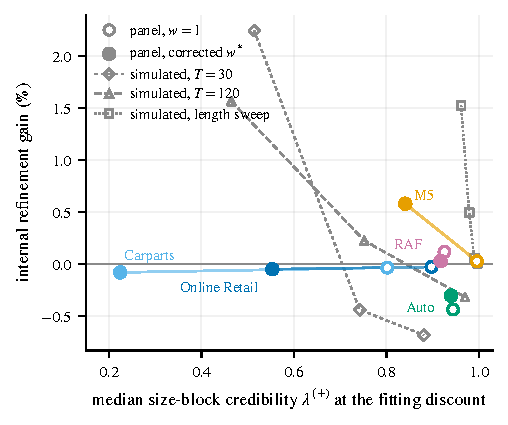
\includegraphics[width=\columnwidth]{figs/fig10a_refinement_leverage_size.pdf}\\[0.5em]
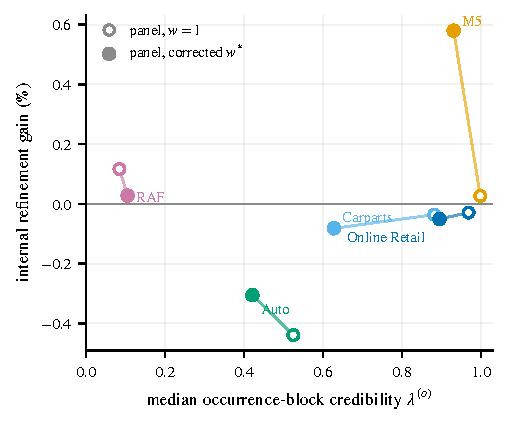
\includegraphics[width=\columnwidth]{figs/fig10b_refinement_leverage_occ.pdf}
\caption{\textbf{The simulated curves are an upper envelope that the real
panels do not reach.} Internal refinement gain (best refined structure
versus the global pool, validation SPL) against median credibility weight,
on the size block (top) and the occurrence block (bottom). Open markers
are $w{=}1$, filled markers the selected discount, and the connecting
segment is the movement forgetting induces. Grey curves are the controlled
panels of Section~\ref{sec:synthetic}, where the partition supplied is
correct by construction. % [ORIG 2026-09-13]
The grey curves pool the three separations of the
controlled grid; Figure~\ref{fig:separation} resolves them. Read against
the pooled envelope, every real panel lies below it at its own leverage.}
\label{fig:refinement-leverage}
\end{figure}


\paragraph{High leverage is an amplifier with no sign attached.}
The clearest illustration is RAF, which combines the highest size-block
leverage in the panel set ($\lambda^{(+)}=0.917$) with the lowest
occurrence leverage ($\lambda^{(o)}=0.106$), and loses $31.5\%$ of
external MAE to a learned partition. The two facts are one fact. The point
forecast is $\hat y_i=\hat\pi_i\exp(\hat\mu_i+\hat\sigma_i^2/2)$; when
$89\%$ of $\hat\pi_i$ comes from the group prior, replacing the group is
close to replacing the forecast. This is the empirical content of the
caveat attached to Proposition~\ref{prop:active}: persistent prior leverage
guarantees that the choice of target keeps mattering, not that a
particular target is good. Read together with the previous paragraph, low
leverage caps the upside and high leverage uncaps the downside, and
neither makes a learned partition worth using here.

\begin{table}[t]
\centering
\caption{Online Retail distributional ablation. Each row is an
independent hierarchical run; ``auto'' denotes its own internal discount
selection. The raw predictive law is used and lower is better. Full
point metrics are in Appendix Table~\ref{tab:ablation-full}.}
\label{tab:ablation}
\small
\begin{tabular*}{\columnwidth}{@{\extracolsep{\fill}}llrrr@{}}
\toprule
Pooling & Forget & SPL & SPL$_{90}$ & AIW\\
\midrule
global & off & 0.8899 & 1.5306 & 10.51\\
taxonomy & off & 0.8897 & 1.5299 & 10.56\\
learned & off & 0.8905 & 1.5336 & 10.79\\
global & auto ($.95$) & \secondbest{0.8849} & \secondbest{1.5268} & \best{9.25}\\
taxonomy & auto ($.95$) & \best{0.8846} & \best{1.5254} & 9.43\\
learned & auto ($.95$) & 0.8869 & 1.5343 & 10.69\\
\bottomrule
\end{tabular*}
\end{table}

\paragraph{What the ablation confirms.}
Table~\ref{tab:ablation} is the external counterpart on Online Retail: the
three pooling candidates differ by less than $0.1\%$ in mean SPL without
forgetting and by less than $0.3\%$ at the selected discount, matching the
internal picture. Discounting shows up
elsewhere, narrowing the global and taxonomy $80\%$ intervals by
$11$--$12\%$ while improving mean SPL by about half a percent; the full
ablation
(Appendix Table~\ref{tab:ablation-full}) shows it improves external MAE by
$3.5$--$4.0\%$ and slightly worsens RMSE. The cross-panel result in
Table~\ref{tab:prob} should therefore be attributed to the shared
hurdle-EB predictive law and to the temporal half of the selection, not to
a learned-partition gain. That is not a concession made after the fact:
the leverage diagnostic states the ceiling in advance, and
Figure~\ref{fig:refinement-leverage}\ shows we do not reach it.


\subsection{Pre-fit screen: protocol, metrics, and real-series transfer}
\label{app:room}

\begin{figure*}[t]
\centering
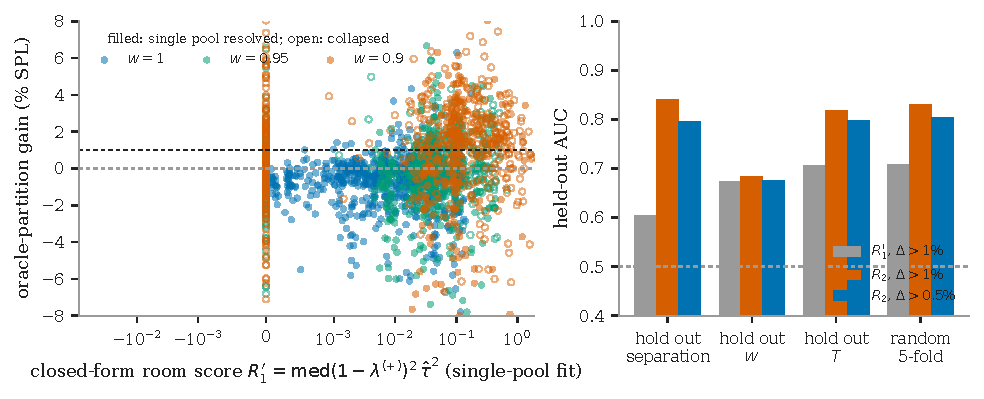
\includegraphics[width=0.96\textwidth]{figs/fig15_room_diagnostic.pdf}
\caption{\textbf{Screening for pooling room before any partition is
fitted.} Left: the closed-form score computed from the single-pool fit
against the oracle partition's realized gain on $2{,}700$ simulated
panels, colored by discount; open markers are panels whose single-pool
variance component collapsed. Right: held-out AUC for the event that the
oracle gain exceeds one percent (or half a percent), when whole
separation levels, discounts, or lengths are held out, or under random
folds; $R_1'$ is the closed-form score and $R_2$ a logistic screen on the
same fitting-window quantities.}
\label{fig:room}
\end{figure*}


\paragraph{Protocol.} The grid crosses separation $\{0,.25,.5,1,2\}$,
discount $\{1,.95,.90\}$, length $\{30,60,120\}$, occurrence mean
$\{.1,.25,.5\}$, items per group $\{20,60\}$, and balanced versus
$70/10/10/10$ group sizes, with four groups, $\tau^2=0.15$, $\sigma^2=1$,
occurrence separation scaled as $0.8\min(\mathrm{sep},1)$, five
replicates per cell, and seed 20260915. Per panel, only the single-pool
fit is used for features: median retained leverage on the size and
occurrence blocks, $\hat\tau^2$, the Beta concentration, the resolution
statistic, effective counts, and panel size. The target is the oracle
partition's paired pinball gain over the single pool (estimated
hyperparameters, true labels), which can be negative. The pre-registered
closed-form score $R_1$ used an unweighted mean of sampling variances
that is dominated by items whose discounted positive count approaches
zero; it has no screening power (AUC $0.45$--$0.64$) and is retained in
the released artifact. $R_1'$ replaces that term by the pool's own
weighted estimate $\hat\tau^2$; $R_2$ is a logistic regression on
$\log(1+\cdot)$ of the features, fitted on the training folds only. The
design, the amendments, and their order are recorded in
\texttt{docs/DESIGN\_room\_diagnostic.md}.

\begin{table}[t]
\centering
\caption{Held-out screening performance on the simulated grid for the
event that the oracle partition's gain exceeds one percent (base rate
$22\%$). Columns: AUC of the pre-registered $R_1$, of $R_1'$, and of the
logistic screen $R_2$ on all panels; the same for $R_1'$ and $R_2$ on the
panels whose single-pool variance component did not collapse; precision
and recall of $R_2$ at its best-$F_1$ threshold.}
\label{tab:room}
\small
\setlength{\tabcolsep}{3.5pt}
\begin{tabular}{lcccccc}
\toprule
 & \multicolumn{3}{c}{All panels} & \multicolumn{2}{c}{Resolved} & \\
\cmidrule(lr){2-4}\cmidrule(lr){5-6}
Held out & $R_1$ & $R_1'$ & $R_2$ & $R_1'$ & $R_2$ & $R_2$ P / R\\
\midrule
hold out a separation level & 0.45 & 0.60 & 0.84 & 0.72 & 0.85 & 0.54 / 0.77\\
hold out a discount & 0.64 & 0.67 & 0.68 & 0.66 & 0.68 & 0.51 / 0.49\\
hold out a length & 0.51 & 0.71 & 0.82 & 0.79 & 0.83 & 0.54 / 0.67\\
random 5-fold & 0.51 & 0.71 & 0.83 & 0.78 & 0.84 & 0.55 / 0.65\\
\bottomrule
\end{tabular}
\end{table}

\paragraph{Real-series transfer.} Online Retail, Carparts, and the
5{,}000-series M5 sample keep their zeros, noise, lengths, and scales; a
known partition is injected by multiplying every positive value of item
$i$ by $\exp(\delta_{g(i)})$ with symmetric offsets
$\{\pm0.5,\pm1.5\}\times\delta$, $\delta\in\{0,.25,.5,1,2\}$, over four
randomly assigned groups (three assignments), at the selected discount and
again at $w=0.90$. The oracle gain of the injected partition never exceeds
0.4\% on any panel: the single pool absorbs the injected
heterogeneity ($\hat\tau^2$ rises from $0.04$ to $5.1$ on Carparts as
$\delta$ goes from $0$ to $2$) and the median size-block credibility
rises toward one, so the items' own evidence, not the prior, carries the
forecast. $R_2$, fitted on the simulated grid and applied unchanged,
assigns every injected panel a probability below 0.17 of material
room (Figure~\ref{fig:room-transfer}). The transfer test therefore checks
the screen's rejections, not its detections; a real-series test of
detections would require panels whose items lack positive observations,
which is the short-history regime of Section~\ref{sec:pays}.

\begin{figure}[t]
\centering
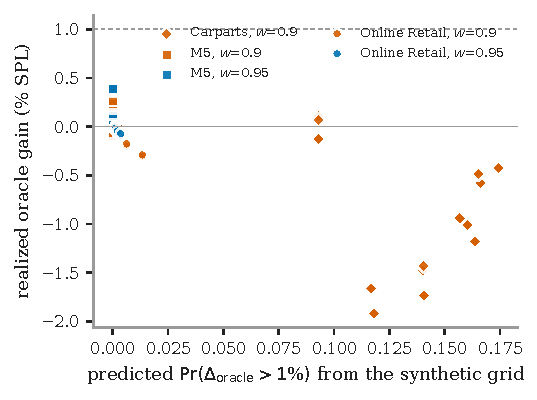
\includegraphics[width=0.9\linewidth]{figs/fig16_room_transfer.pdf}
\caption{Real-series transfer of the screen: predicted probability of
material room (from the simulated grid) against the realized oracle gain
of the injected partition, by panel and discount.}
\label{fig:room-transfer}
\end{figure}

